% ─────────────────────────────────────────────────────────────────────────────
\chapter{Theory}
\label{sec:theory}
% ─────────────────────────────────────────────────────────────────────────────

SUN-DIC implements local (subset-based) Digital Image Correlation
\citep{Sutton2009, Pan2018}, in which the image is divided into small overlapping
subsets that are independently tracked from a reference image to a deformed image.
The sections below provide a short summary of some of the key algorithmic components implemented in SUN-DIC. A good high level overview of DIC is provided by \href{https://digitalimagecorrelation.org/}{A practical guide to DIC}, while many excellent textbooks and academic papers are available for further reading.

\begin{grayquote}
	The purpose of this chapter is to provide a brief overview of the algorithms implemented in SUN-DIC. It is not intended to be a comprehensive introduction to Digital Image Correlation. Readers interested in detailed derivations and theoretical background are encouraged to consult the references cited throughout this chapter.
\end{grayquote}

% ─────────────────────────────────────────────────────────────────────────────
\section{The DIC Problem}

Let $f(\mathbf{x})$ be the intensity at pixel $\mathbf{x} = (x, y)$ in the reference
image and $g(\mathbf{x}')$ the intensity at the corresponding location in the deformed
image. A subset $S$ centred at $\mathbf{x}_0$ in the reference image is mapped to the
deformed image by a warp function $\mathcal{W}(\boldsymbol{\xi};\,\mathbf{p})$,
where $\boldsymbol{\xi} = (\xi,\eta)$ are local coordinates measured relative to the
subset centre and $\mathbf{p}$ is the vector of deformation parameters
(see Section~\ref{sec:shape}).

The goal of the optimisation is to determine the deformation parameters $\mathbf{p}$
that best align the reference subset with its counterpart in the deformed image by
minimising a correlation cost function.

% ─────────────────────────────────────────────────────────────────────────────
\section{Correlation Criterion}
\label{sec:znssd}

Many correlation criteria have been proposed in the DIC literature. SUN-DIC uses the
Zero-Mean Normalised Sum of Squared Differences (ZNSSD) criterion to determine the
optimal deformation parameters $\mathbf{p}$.  The ZNSSD criterion provides robustness to illumination changes by normalising intensity values within each subset:

\begin{equation}
	\label{eqn:znssd}
	C_\text{ZNSSD}(\mathbf{p}) =
	\sum_{\boldsymbol{\xi} \in S}
	\left[
	\frac{f(\mathbf{x}_0+\boldsymbol{\xi}) - \bar{f}}{\Delta f}
	-
	\frac{g\!\left(\mathcal{W}(\boldsymbol{\xi};\mathbf{p})\right) - \bar{g}}{\Delta g}
	\right]^2
\end{equation}
where $\bar{f}$ and $\bar{g}$ are the mean intensities of the reference and deformed
subsets, and

\begin{equation}
	\Delta f = \sqrt{\sum_{\boldsymbol{\xi} \in S}
		\bigl(f(\mathbf{x}_0+\boldsymbol{\xi}) - \bar{f}\bigr)^2},
	\qquad
	\Delta g = \sqrt{\sum_{\boldsymbol{\xi} \in S}
		\bigl(g\bigl(\mathcal{W}(\boldsymbol{\xi};\mathbf{p})\bigr) - \bar{g}\bigr)^2}
\end{equation}
are the $L_2$ norms of the zero-mean subsets. ZNSSD is insensitive to uniform changes in illumination offset and scale.

The closely related Zero-Mean Normalised Cross-Correlation (ZNCC) is related to ZNSSD by \citep{Pan2013a}:

\begin{equation}
	\label{eqn:zncc}
	\text{ZNCC} = 1 - \tfrac{1}{2}\,C_\text{ZNSSD}
\end{equation}

The ZNCC value ranges from $-1$ to $1$, where a value of $1$ indicates a perfect match between the reference and deformed subsets. SUN-DIC uses ZNCC as an optional convergence criterion via the \code{NZCCThreshold} parameter.

% ─────────────────────────────────────────────────────────────────────────────
\section{Subpixel Interpolation}

Deformation rarely produces integer-pixel shifts, so the deformed subset intensities
must be evaluated at non-integer pixel locations at every optimisation iteration.
Accurate subpixel interpolation is essential for measurement accuracy
\citep{Schreier2000}.

SUN-DIC uses bicubic (\code{InterpolationOrder=3}) or biquintic (\code{InterpolationOrder=5}) interpolation \citep{fast_interp}. Fifth-order interpolation is marginally more accurate, while third-order interpolation is generally more numerically robust and is recommended for most applications.

% ─────────────────────────────────────────────────────────────────────────────
\section{Shape Functions}
\label{sec:shape}

The mapping between the reference and deformed subsets is described by a shape function that approximates the local deformation within each subset. SUN-DIC supports both affine and quadratic shape functions.

\subsection{Affine Shape Functions (6~DOF)}

The affine warp uses six deformation parameters and is written in homogeneous matrix form \citep{Gao2015}:

\begin{equation}
	\label{eqn:affine}
	\mathcal{W}(\boldsymbol{\xi};\,\mathbf{p})
	=
	\begin{bmatrix}
		1+u_x & u_y   & u \\
		v_x   & 1+v_y & v \\
		0     & 0     & 1
	\end{bmatrix}
	\begin{pmatrix} \xi \\ \eta \\ 1 \end{pmatrix}
\end{equation}
with $\mathbf{p} = (u,\,u_x,\,u_y,\,v,\,v_x,\,v_y)^T$, where $(u, v)$ are the in-plane translations and $(u_x,\,u_y,\,v_x,\,v_y)$ are first-order displacement gradients that capture uniform stretching, rotation, and shear within the subset. Figure~\ref{fig:affine_theory} illustrates the transformation.

\begin{figure}[!hbt]
	\centering
	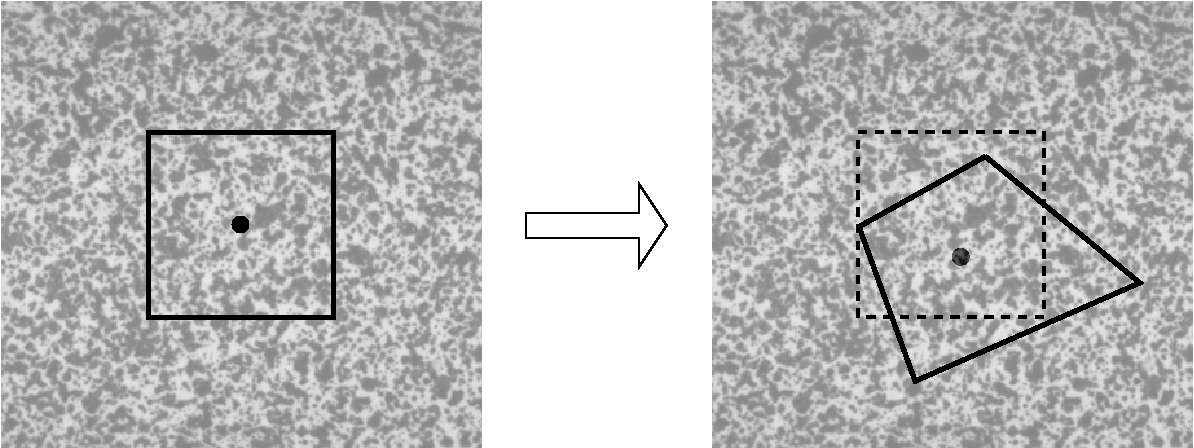
\includegraphics[width=9cm]{figures/affine-crop.pdf}
	\caption{Affine transformation from reference (left) to deformed (right) subset.}
	\label{fig:affine_theory}
\end{figure}

\subsection{Quadratic Shape Functions (12~DOF)}

The quadratic warp adds second-order terms, increasing the parameter vector to

\[
\mathbf{p} = (u,\,u_x,\,u_y,\,u_{xx},\,u_{xy},\,u_{yy},\,
v,\,v_x,\,v_y,\,v_{xx},\,v_{xy},\,v_{yy})^T.
\]

This model can better represent non-uniform deformation, bending, and large strain gradients. However, the additional degrees of freedom increase sensitivity to noise and generally require larger subset sizes for stable results.


\section{Optimisation Algorithms}

SUN-DIC provides two optimisation algorithms for determining the deformation parameters $\mathbf{p}$.
Both are based on the inverse compositional framework \citep{Baker2001, Pan2013a}, where image gradients and the Hessian are computed once from the reference image and reused at every iteration, providing significant computational savings.

The approximate Hessian is

\begin{equation}
	\label{eqn:hessian}
	\mathbf{H} = \sum_{\boldsymbol{\xi} \in S}
	\mathbf{s}(\boldsymbol{\xi})^T\,\mathbf{s}(\boldsymbol{\xi})
\end{equation}
with

\begin{equation}
	\mathbf{s}(\boldsymbol{\xi})
	= \frac{1}{\Delta f}\,
	\nabla f(\mathbf{x}_0+\boldsymbol{\xi})\cdot
	\frac{\partial \mathcal{W}}{\partial \mathbf{p}}\bigg|_{\mathbf{p}=\mathbf{0}}
\end{equation}
where $\nabla f = \bigl(\partial f/\partial x,\;\partial f/\partial y\bigr)$ is the reference-image gradient and $\partial\mathcal{W}/\partial\mathbf{p}$ is the warp Jacobian.

% ─────────────────────────────────────────────────────────────────────────────
\subsection{IC-GN: Inverse Compositional Gauss--Newton}
\label{sec:icgn}

The IC-GN algorithm computes the residual:

\begin{equation}
	r(\boldsymbol{\xi};\mathbf{p}) =
	\frac{f(\mathbf{x}_0+\boldsymbol{\xi}) - \bar{f}}{\Delta f}
	-
	\frac{g\!\left(\mathcal{W}(\boldsymbol{\xi};\mathbf{p})\right) - \bar{g}}{\Delta g}
\end{equation}
The parameter update is

\begin{equation}
	\label{eqn:icgn}
	\Delta\mathbf{p} = -\,\mathbf{H}^{-1}
	\sum_{\boldsymbol{\xi} \in S}
	\mathbf{s}(\boldsymbol{\xi})^T\,r(\boldsymbol{\xi};\mathbf{p})
\end{equation}
and the warp update is

\begin{equation}
	\label{eqn:warp_update}
	\mathcal{W}(\cdot;\mathbf{p})
	\;\leftarrow\;
	\mathcal{W}(\cdot;\mathbf{p}) \circ \mathcal{W}(\cdot;\Delta\mathbf{p})^{-1}
\end{equation}

IC-GN exhibits second-order convergence near the solution but has a relatively limited convergence radius. Reliable initial guesses (Section~\ref{sec:start}) are therefore important for robust performance.

% ─────────────────────────────────────────────────────────────────────────────
\subsection{IC-LM: Inverse Compositional Levenberg--Marquardt}
\label{sec:iclm}

IC-LM replaces the Hessian with a damped form:

\begin{equation}
	\label{eqn:iclm}
	\Delta\mathbf{p} = -\,(\mathbf{H} + \lambda\mathbf{I})^{-1}
	\sum_{\boldsymbol{\xi} \in S}
	\mathbf{s}(\boldsymbol{\xi})^T\,r(\boldsymbol{\xi};\mathbf{p})
\end{equation}

The damping parameter $\lambda$ is adapted dynamically to balance stability and speed. This gives IC-LM a larger convergence radius than IC-GN, although each iteration is computationally more expensive.

SUN-DIC also provides an experimental \code{Fast-IC-LM} variant that improves computational efficiency while introducing only a negligible loss in accuracy.

\textbf{Guidance:} IC-GN with AKAZE initialisation (Section~\ref{sec:start}) is sufficient for most cases. IC-LM is recommended for difficult cases involving large deformation gradients or poor initial guesses.

% ─────────────────────────────────────────────────────────────────────────────
\section{Starting Strategy -- AKAZE Initialisation}
\label{sec:start}

Both IC-GN and IC-LM require good initial estimates for $\mathbf{p}$ to converge reliably. SUN-DIC uses a two-phase strategy to generate robust initial guesses and reduce the risk of error propagation between neighbouring subsets.

\textbf{Phase 1 -- Initialisation:} An $n \times n$ grid of seed points (controlled by \texttt{StartingPoints}) is distributed across the ROI. For each seed, AKAZE features \citep{Alcantarilla2013} are used to estimate an initial affine transformation and compute $C_\text{ZNSSD}$.

\textbf{Phase 2 -- Propagation:} The best seed is optimised first. Its solution is then propagated to neighbouring subsets, and optimisation proceeds in order of increasing initial cost function values. This reduces the accumulation of errors that can occur in purely sequential approaches.

AKAZE is preferred for its robustness to blur, rotation, scaling, and affine distortions \citep{Isik2024}.


\section{Strain Calculation}
\label{sec:strain}

Strains are computed from the displacement field $(u, v)$ produced by the optimiser and are evaluated as a post-processing step. Because DIC displacement fields contain noise, direct numerical differentiation would amplify errors.  Instead, SUN-DIC applies 2D Savitzky--Golay smoothing \citep{Pan2007a}. The displacement field is locally approximated by a polynomial, and derivatives are computed analytically from the fitted coefficients.

\newpage
The in-plane engineering strains are:

\begin{equation}
	\label{eqn:strains}
	\varepsilon_{xx} = \frac{\partial u}{\partial x}, \qquad
	\varepsilon_{yy} = \frac{\partial v}{\partial y}, \qquad
	\varepsilon_{xy} = \frac{1}{2}\!\left(
	\frac{\partial u}{\partial y} + \frac{\partial v}{\partial x}
	\right)
\end{equation}

The Von Mises equivalent strain is:

\begin{equation}
	\label{eqn:vonmises}
	\varepsilon_\text{VM} =
	\sqrt{
		\varepsilon_{xx}^2
		+ \varepsilon_{yy}^2
		- \varepsilon_{xx}\,\varepsilon_{yy}
		+ 3\,\varepsilon_{xy}^2
	}
\end{equation}
